
\chapter{Introduction to One-Parameter Bifurcation Problems}\label{chap1}


\section{Introduction}\label{chap1-sec1}

In\pageoriginale this, section, we introduce one-parameter bifurcation problems\break through the example of linear eigenvalue problems. In increasing order of generality, they first lead to non-linear eigenvalue problems, next, to problems of bifurction from the trivial branch and finally to a large class of problems for which a general mathematical analysis can be developed.

\subsection{Linear Eigenvalue Problems}\label{chap1-subsec1.1a}

Let $X$ be a real vector space. Given a linear operator $L : X \to X$, we consider the problem of finding the pairs $(\lambda, x) \epsilon \mathbb{R} \times X$ that
$$
x = \lambda L x.
$$

For $\lambda = 0, x = 0$ is the unique solution. For $\lambda \neq 0$, and setting $\tau = 1 / \lambda$, it is equivalent to
$$
\tau x = L x.
$$

The values $\tau \epsilon \mathbb{R}$ such that there exists $x \neq 0$ satisfying the above equation are called {\em eigen values} of $L$. When $\lambda \neq 0$, the corresponding value $\lambda = 1/\tau$ is called a {\em characteristic value } of $L$.

It may happen that every non-zero real number $\lambda$ is a characteristic\pageoriginale value of $L$. For instance, if $X = \mathscr{D}' (\mathbb{R})$ (distributions over $\mathbb{R}$) and $L$ is the operator $Lx = x'' \epsilon \mathscr{D} (\mathbb{R})$. Then
$$
x = \lambda x'' \leftrightarrow x(s) = e^{s / \surd \lambda}.
$$

But this is not the case in general. In what follows, we shall assume that $X$ is a real {\em Banach} space and that $L \epsilon \mathscr{L} (x)$ is {\em compact}.

From the {\em special theory of linear operators} in Banach spaces, it is known that
\begin{enumerate}
\item[(i)] The characteristic values of $L$ form a sequence $\{\lambda_{j}\}_{ j\geq 1}$ with no cluster point (the sequence is finite if $\dim X < \infty$).

\item[(ii)] For every $\lambda \epsilon \mathbb{R}$, Range $(I - \lambda L)$ is closed and $\dim \Ker (I - \lambda L)$ = codim Range $(I - \lambda L) < \infty$ (and is greater than or equal to 1 if and only if $\lambda = \lambda_{j}$ for some $j$).
\end{enumerate}

Let us now set
$$
H(\lambda, x) = x - \lambda L x
$$
so that the problem consists in finding the pairs $(\lambda, x) \epsilon \mathbb{R} \times X$ such that $H(\lambda, x) = 0$. The set of solutions of this equation ({\em zero set} of $H$) is the union of the line $\{(\lambda, 0) ; \lambda \epsilon \mathbb{R} \}$ ({\em trivial branch}) and the set $\bigcup\limits_{j \geq 1} \{\lambda_{j}\} \times E_{j}$ where $E_{j}$ denotes the eigenspace associated with the characteristic value $\lambda_{j}$.

Now, let us take a look at the local structure of the zero set\pageoriginale of H around a given point $(\lambda_{0}, 0), \lambda_{0} \epsilon \mathbb{R}$ ; If $\lambda_{0}$ is {\em not} a characteristic value of $L$, it is made up of exactly {\em one} curve (the trivial branch itself). If $\lambda_{0} = \lambda_{j}$ for some $j \geqq 1$, the structure changes, since there are solutions of the form $(\lambda_{j}, x), x \epsilon E_{j}$, arbitrarily close to $(\lambda_{j}, 0)$. The existence of {\em nontrivial} solutions (i.e. which do not belong to the trivial branch) around a point $(\lambda_{j}, 0)$ is referred to as a {\em bifurcation phenomenon} (here, form the trivial branch) and the points $(\lambda_{j}, 0)$ are called {\em bifurction points}. Bifurcation can be viewed as a {\em breaking of smoothess} of the local zero set whereas data whereas {\em all the data are smooth}.

\subsection{Generalization I: Problems of bifurcation from the trivial branch.}\label{chap1-subsec1.1b}

A natural extension is when the linear operator $L$ is replaced by a mapping $T : X \to X$ (nonlinear in general) such that $T(0) = 0$. The problem becomes: Find $(\lambda, x) \epsilon \mathbb{R} \times X$ such that
$$
x = \lambda T(x).
$$

Again, the pairs $(\lambda, 0) \lambda \epsilon \mathbb{R}$ are always solutions of this equation ({\em trivial branch}). On the basis of the linear case, a natural question is to know whether there are {\em ``bifurcation points''} on the trivial branch, namely solutions $(\lambda_{\circ}, 0)$ around which nontrivial solutions always exist.

\begin{theorem}[Necessary condition]\label{chap1-thm1.1}
 Assume that $T$ is differentiable at\pageoriginale the origin and the linear operator $DT(0) \epsilon \mathscr{L} (X)$ is compact. Then a necessary condition for $(\lambda_{0}, 0)$ to be a bifurcation point of the equation $x = \lambda T(x)$ is that $\lambda_{0}$ is a characteristic value of $DT(0)$.
\end{theorem}

\begin{proof}
Write
$$
T(x) = DT(0) \cdot x + \circ(||x||)
$$
and let $(\lambda^{(i)} , x^{(i)})$ be a sequence tending to $(\lambda_{0}, 0)$ with $x^{(i)} \neq 0$ and
$$
x^{(i)} = \lambda^{(i)} T(x^{(i)}).
$$

Thus,
$$
x^{(i)} = \lambda^{(i)} DT(0) \cdot x^{(i)} + 0(||x^{(i)}||)
$$

Dividing by $||x^{(i)}|| \neq 0$, we get
$$
\frac{x^{(i)}}{||x^{(i)}||} = \lambda^{(i)} DT(0). \frac{x^{(i)}}{||x^{(i)}||} + 0(1)
$$

The sequence $\left(\frac{x^{(i)}}{||x^{(i)}||}\right)$ is bounded. Due to the compactness of the operator $DT(0)$, we may assume, after considering a subsequence, that the right hand side tends to a limit $v$, which is then the limit of the sequence $\left(\frac{x^{(i)}}{||x^{(i)}||}\right)$ as well. Of course, $v \neq 0$ and making $i$ tend to $+ \infty$, we find
$$
v = \lambda_{0} DT(0) \cdot v,
$$
which shows that $\lambda_{0}$ is a characteristic value of $DT(0)$.
\end{proof}

\begin{remark}\label{chap1-rem1.1}
As\pageoriginale T is nonlinear (a very general assumption !) it is impossible, without additional hypotheses to expect more than {\em local results} (in contrast to the linear case where global results are obtained).
\end{remark}

\begin{remark}\label{chap1-rem1.2}
Even when $\lambda_{0}$ is a characteristic value of $DT(0)$, bifurcation is not ensured. For instance, take $X = \mathbb{R}^{2}$ and $x = (x_{1}, x_{2})$ with
\begin{equation*}
T(x_{1}, x_{2}) = 
\begin{bmatrix}
x_{1}  + x_{2}^{3}\\[4pt]
x_{2}  -  x_{1}^{3}
\end{bmatrix}.
\end{equation*}

Here, $DT(0) = I$ , whose unique characteristic value is $\lambda_{1} = 1$. The equation $x = \lambda T(x)$ becomes
\begin{align*}
x_{1} & = \lambda x_{1} + \lambda x_{2}^{3},\\
x_{2} & = \lambda x_{2} - \lambda x_{1}^{3}.
\end{align*}
Multiplying the first equation by $x_{2}$ and the second one by $-x_{1}$ and adding the two we get $\lambda(x_{1}^{4} + x_{2}^{4}) = 0$. Hence for $\lambda$ around 1, we must have $x = 0$ and {\em no bifurcation occurs.}
\end{remark}

These nonlinear eigenvalue problems are particular cases of a more general class called {\em problems of bifurcation from the trivial branch}. By {\em definition}, a problem of bifurcation from the trivial branch is an equation of the form
$$
x = \lambda L x - \phi (\lambda, x),
$$
where $L \epsilon \mathscr{L}(X)$ and $\phi$ is a nonlinear operator from $X$ to itself satisfying\pageoriginale
\begin{align*}
\phi (\lambda, 0) & = 0 \text{ for } \lambda \epsilon \mathbb{R},\tag{1.1}\label{chap1-eq1.1}\\
\phi (\lambda, x) & = 0(||x||),\tag{1.2}\label{chap1-eq1.2}
\end{align*}
for $x$ around the origin, {\em uniformly with respect to $\lambda$ on bounded intervals}. It is equivalent to saying that a problem of bifurcation from the trivial branch consists in finding the zero set of the mapping
$$
H(\lambda, x) = x - \lambda L x + \phi (\lambda, x)
$$

From our assumptions, the pairs $(\lambda, 0), \lambda \epsilon \mathbb{R}$ are all in the zero set of $H$ ({\em trivial branch}). Note, however, that our definition does {\em not} include all mappings having the trivial branch in their zero set. Two reasons motivate our definition. First, problems of this type are common in the literature, for they correspond to many physical examples. Secondly, from a mathematical stand-point, their properties allow us to make a general study of their zero set. In particular, when $L$ is {\em compact}, a proof similar to that of theorem \ref{chap1-thm1.1} shows that $\lambda_{0}$ needs to be characteristic value of $L$ for $(\lambda_{0}, 0)$ to be a bifurcation point. Actually, by writing the Taylor expansion of $T$ about the origin
$$
T(x) = DT(0) \cdot x + R(x),
$$
with $R(x) = 0(||x||)$, it is clear that nonlinear eigenvalue problems are a particular case of problems of bifurcation from the trivial branch in which $L = DT(0)$ and $\phi(\lambda, x) = -\lambda R(x)$.

The\pageoriginale most famous result about problems of bifurction from the trivial branch is a partial converse of Theorem \ref{chap1-thm1.1} due to Kranoselskii.

\begin{theorem}[Krasnoselskii]\label{chap1-thm1.2}
Assume that $L$ is compact and $\lambda_{0}$ is a characteristic value of $L$ with odd algebraic multiplicity, Then $(\lambda_{0}, 0)$ is a bifurcation point (i.e. there are solutions $(\lambda, x) \epsilon \mathbb{R} \times X - \{0\}$ of $H(\lambda, x) = 0$ arbitrarily close to $(\lambda_{0}, 0)$).
\end{theorem}

The proof of Theorem \ref{chap1-thm1.2} is based on {\em topological degree arguments} and will not be given here (cf. \cite{19}, \cite{27}). It is a very general result but it does not provide any information on the {\em structure} of the zero set of $H$ near $(\lambda_{0}, 0)$, a question we shall be essentially interested in, throughout these notes.

\begin{comment}\label{chap1-com1.1}
(Algebraic and geometric multiplicity of a characteristic value): Let $L$ be compact. Given a characteristic value $\lambda_0$ of $L$, it is well-known that the space $\Ker (I - \lambda_{0} L)$ is finite dimensional. Its dimension is called the {\em geometric multiplicity} of $\lambda_{0}$.
\end{comment}

The spectral theory of compact operators in Banach spaces (see e.g. \cite{9}) provides us with additional information; namely, there is an integer $r \geq 1$ such that
\begin{enumerate}
\item[(i)] $\dim \Ker (I - \lambda_{0} L)^{r} < \infty$,

\item[(ii)] $X = \Ker(I - \lambda_{0} L)^{r} \oplus Range (I - \lambda_{0} L)^{r}$.
\end{enumerate}

In\pageoriginale addition, $r$ is characterized by
$$
\Ker (I - \lambda_{0} L)^{r'} = \Ker(I - \lambda_{0} L)^{r} \text{ for every } r' \geq r.
$$

The dimension of the space $\Ker (I - \lambda_{0}L)^{r}$ is called the {\em algebraic multiplicity} of $\lambda_{0}$. The algebraic multiplicity of $\lambda_{0}$ is always greater holds if an only if $r = 1$. If so, it follows from property (ii) that
$$
X = \Ker(I - \lambda_{0}L) \oplus Range (I - \lambda_{0}L).
$$

A typical example of this situation is when $X$ is a Hilbert space and $L$ is {\em self-adjoint}.

\begin{comment}\label{chap1-com1.2}
In particular, Krasnoselskii's theorem applied when $r = 1$ and $\dim \Ker (I - \lambda_{0}L) = 1$. For instance, this happens when $L$ is the inverse of a {\em second order} elliptic linear operator associated with suitable boundary conditions and $\lambda_{0}$ is the ``first'' characteristic value of $L$; this result is strongly related to the {\em maximum principle} through the Krein-Rutman theorem. (See e. g. \cite{20, 35}).
\end{comment}

\begin{comment}\label{chap1-com1.3}
For future use, note that the mapping $\phi$ is differentiable with respect to the $x$ variable at the origin with
\begin{equation*}
D_{x} \phi (\lambda, 0) = 0 \text{ for every } \lambda \epsilon \mathbb{R},\tag{1.3}\label{chap1-eq1.3}
\end{equation*}
as it follows from (\ref{chap1-eq1.2}).
\end{comment}


\begin{examples*}
The most important examples of problems of bifurcation from the trivial branch came from nonlinear partial differential equations.\pageoriginale For instance, let us consider the model problem
\begin{equation*}
\begin{cases}
- \triangle u + \lambda u \pm u^{k} = 0 \text{ in } \Omega,\\
u \epsilon H_{0}^{1} (\Omega),
\end{cases}
\end{equation*}
where $\Omega$ is a bounded open subset of $\mathbb{R}^{N}$ and $k \geq 2$ is an integer.
\end{examples*}

Under general assumptions on the boundary $\partial \Omega$ of $\Omega$, it follows from the {\em Sobolev embedding theorems} that $u^{k} \epsilon H^{-1} (\Omega)$ for $k \leq \frac{N+2}{N-2}$ if $N > 2$, any $1 \leq k < + \infty$ for $N = 1$ and $N = 2$.

Denoting by $L \epsilon \mathscr{L} (H^{-1} (\Omega), H_{0}^{1} (\Omega))$ the inverse of the operatoe $-\triangle$, the problem becomes equivalent to
\begin{equation*}
\begin{cases}
u - \lambda L u + L(u^{k}) = 0,\\
u \epsilon H_{0}^{1} (\Omega).
\end{cases}
\end{equation*}

Note that the restriction of $L$ to the space $H_{0}^{1} (\Omega)$ is compact and the mapping
$$
u \epsilon H_{0}^{1} (\Omega) \to Lu^{k} \epsilon H_{0}^{1} (\Omega)
$$
is of class $C^{\infty}$. In this example, the nonlinearity $u^{k}$ can be replaced by $F(u)$ (respectively $F(\lambda, u)$) where $F(u)(x) = f(x, u(x))$ (respectively $F(\lambda, u)(x) = f(\lambda, x, u(x))$) and $f$ is a {\em Carath\'{e}odory} function satisfying some suitable growth conditions with respect to the second (respectively third) variable (see eg. Krasnoselskii \cite{19}, Rabier \cite{30}).

Another\pageoriginale example with a {\em non-local nonlinearity} is given by the {\em von Karman equations} for the study of the buckling of thin plates. The problem reads: Find $u$ such that
\begin{equation*}
\begin{cases}
u - \lambda L u + C(u) = 0,\\
u \epsilon H_{0}^{2} (\omega),
\end{cases}
\end{equation*}
where $\omega$ is an open bounded subset of the plane $\mathbb{R}^{2}$, $L \epsilon \mathscr{L} (H_{0}^{2} (\omega))$ is compact and $C$ is a ``cubic'' nonlinear operator. The operator $L$ takes into account the distribution of lateral forces along the boundary $\partial \omega$, the intensity of these forces being proportional to the scalar $\lambda$. For ``small'' values of $\lambda$, the only solution is $u = 0$ but, beyond a certain critical value, nonzero solutions appear: this corresponds to the (physically observed) fact that the plate jumps out of its for sufficiently ``large'' $\lambda$ (see e. g. Berger \cite{1} Ciarlet-Rabier \cite{6}).

Coming back to the general case, our aim is to give as precise a description as possible of the sero set of $H$ around the point $(\lambda_{0}, 0)$. Assuming $L$ is compact, we already know the answer when $\lambda_{0}$ is not a characteristic value of $L$: the zero set coincides with the trivial branch. In any case, it is convenient to shift the origin and set
\begin{align*}
\lambda & = \lambda_{0} + \mu\tag{1.4}\label{chap1-eq1.4}\\
\Gamma (\mu, x) & = \phi (\lambda_{0} + \mu, x)\tag{1.5}\label{chap1-eq1.5}
\end{align*}
so\pageoriginale that the problem amounts to finding the zero set around the origin (abbreviated as {\em local zero set}) of the mapping
\begin{equation*}
G(\mu, x) = x - (\lambda_{0} + \mu) Lx + \Gamma(\mu, x)\tag{1.6}\label{chap1-eq1.6}
\end{equation*}

Note that the mapping $\Gamma$ verifies the properties
\begin{align*}
\Gamma (\mu, 0) & = 0 \text{ for every } \mu \epsilon \mathbb{R},\tag{1.7}\label{chap1-eq1.7}\\
\Gamma(\mu, x) & = 0(||x||),\tag{1.8}\label{chap1-eq1.8}
\end{align*}
around the origin, {\em uniformly with respect to $\mu$ on bounded intervals}. In particular, $\Gamma$ is differentiable with respect to the $x$-variable and 
\begin{equation*}
D_{x} \Gamma (\mu, 0) = 0 \text{ for every } \mu \epsilon \mathbb{R}.\tag{1.9}\label{chap1-eq1.9}
\end{equation*}

\subsection{GENERALIZATION II :}\label{chap1-subsec1.1c}
Let us consider a problem of bifurcation from the trivial branch with compact operator $L \epsilon \mathscr{L} (X)$, put under the form $G(\mu, x) = 0$ after fixing the real number $\lambda_{0}$ as described above. From (\ref{chap1-eq1.7})
\begin{equation*}
D_{\mu} \Gamma(0) = 0.\tag{1.10}\label{chap1-eq1.10}
\end{equation*}

Together with (\ref{chap1-eq1.9}), we see that the (global) derivative $DG(0)$ is the mapping
\begin{equation*}
(\mu, x) \epsilon \mathbb{R} \times X \to (I - \lambda_{0} L) x \epsilon X.\tag{1.11}\label{chap1-eq1.11}
\end{equation*}

Hence
\begin{align*}
& \Ker DG(0) = \mathbb{R} \times \Ker(I - \lambda_{0} L),\tag{1.12}\label{chap1-eq1.12}\\
& Range DG(0) = Range (I - \lambda_{0}L).\tag{1.13}\label{chap1-eq1.13}
\end{align*}

As\pageoriginale a result, Range $Dg(0)$ is {\em closed} and $\dim \Ker DG(0) = codim\break Range DG(0) + 1 < \infty$ ($\geq 1$, if and only if $\lambda_{0}$ is a characteristic value of $L$). In other words, $DG(0)$ is a {\em Fredholm operator with index} 1. Recall that a linear operator $A$ from a Banach space $\widetilde{X}$ to a Banach space $Y$ is said to be a {\em Fredholm operator} if
\begin{enumerate}
\item[(i)] Range $A$ is closed,

\item[(ii)] $\dim \ker A < \infty$, codim Range $A < \infty$.
\end{enumerate}

In this case, the difference
$$
\dim \Ker A - codim Range A
$$
is called the {\em index} of $A$. For the definition and further properties of Fredholm operators, see Kato \cite{17} or Schecter \cite{36}.

\begin{remark}\label{chap1-rem1.3}
One should relate the fact that the index of $DG(0)$ is 1 to the fact that the parameter $\mu$ is {\em one-dimensional.} This will be made more clear in Remark \ref{chap1-rem2.2} later.
\end{remark}

Although the parameter $\mu$ has often a {\em physical significance} (end hence must be distinguished from the variable $x$ for physical reasons), it is not always desirable to let it play a particular role in the {\em mathematical approach} of the problem.

The suitable general mathematical framework is as follows:

Let there be given two real Banach spaces $\widetilde{X}$ and $Y$ and let $G : \widetilde{X} \to Y$\pageoriginale be a mapping satisfying the conditions
\begin{align*}
& G(0) = 0\tag{1.14}\label{chap1-eq1.14}\\
& G \text{ is differentiable at the origin },\tag{1.15}\label{chap1-eq1.15}\\
& DG(0) \text{ is a Fredholm operator with index 1. }\tag{1.16}\label{chap1-eq1.16}
\end{align*}

Naturally, $G$ need not be defined everywhere, but in a neighbourhood of the origin only. However, for notational convenience, {\em we shall repeatedly make such an abuse of notation} in the future, without further mention.

In our previous example of problems of bifurcation from the trivial branch, one has $\widetilde{X} = \mathbb{R} \times X, Y = X$ and $G(\mu, 0) = 0$ for $\mu \epsilon \mathbb{R}$. None of these assumptions is required here. In particular, nothing ensures that the trivial branch is in the local zero set of $G$. As a matter of fact, {\em no branch of solutions} (trivial or not) {\em is supposed to be known a priori}.

The first step of the study consists in performing the {\em Lyapunov-Schmidt reduction} allowing us to reduce the problem to a {\em finite dimensional one} and this will be done in the next section.

\section{The Lyapunov-Schmidt Reduction}\label{chap1-sec2}

Let $\widetilde{X}$ and $Y$ be two real Banach spaces and $G : \widetilde{X} \to Y$ a mapping of class $C^{m}, m \geq 1$ verifying (\ref{chap1-eq1.14}) - (\ref{chap1-eq1.16}). Let us set
\begin{align*}
& \widetilde{X}_{1} = \Ker DG(0),\tag{2.1}\label{chap1-eq2.1}\\
& Y_{2} = Range DG(0).\tag{2.2}\label{chap1-eq2.2}
\end{align*}\pageoriginale

By hypothesis, $Y_{2}$ has finite codimension $n \geq 0$ as $\widetilde{X}_{1}$ has finite dimension $n + 1$. Let $\widetilde{X}_{2}$ and $Y_{1}$ be two topological complements of $\widetilde{X}_{1}$ and Y respectively.

\begin{remark}\label{chap1-rem2.1}
({\em Existence of topological complements}) From the Hahn-Banach theorem, each one-dimensional subspace of $\widetilde{X}$ has a topological complement. Then, each finite dimensional subspace of $\widetilde{X}$ (direct sum of a finite number of one-dimensional subspaces) has a topological complement (the intersection of the complements of these one-dimensional subspaces). In particular, $\widetilde{X}_{1}$ has a topological complement. Next, the existence of a topological complement of $Y_{2}$ is due to the fact that $Y_{2}$ is {\em closed} with finite codimension. Any (finite-dimensional) algebraic complement of $Y_2$ is closed and hence is also a topological complement. Details are given for instance, in Brezis \cite{4}.
\end{remark}

Thus we can write
\begin{align*}
& \widetilde{X} = \widetilde{X}_{1} \oplus \widetilde{X}_{2}\tag{2.3}\label{chap1-eq2.3}\\
& Y = Y_{1} \oplus Y_{2}.\tag{2.4}\label{chap1-eq2.4}
\end{align*}

Let $Q_{1}$ and $Q_{2}$ denote the (continuous) projection operators onto $Y_{1}$ and $Y_{2}$ respectively. On the other hand, for every $\widetilde{x} \epsilon \widetilde{X}$, set 
$$
\widetilde{x} = \widetilde{x}_{1} + \widetilde{x}_{2}, \widetilde{x}_{1} \epsilon \widetilde{X}_{1}, \widetilde{x}_{2} \epsilon \widetilde{X}_{2}.
$$

With this notation, the equation $G(\widetilde{x}) = 0$ goes over into the system
\begin{align*}
& Q_{1} G(\widetilde{x}_{1} + \widetilde{x}_{2}) = 0 \epsilon Y_{1},\tag{2.5}\label{chap1-eq2.5}\\
& Q_{2} G(\widetilde{x}_{1} + \widetilde{x}_{2}) = 0 \epsilon Y_{2},\tag{2.6}\label{chap1-eq2.6}\\
\end{align*}\pageoriginale

Now, from our assumptions, one has
\begin{equation*}
DG(0) |_{\widetilde{X}_{2}} \epsilon Isom (\widetilde{X}_{2}, Y_{2}).\tag{2.7}\label{chap1-eq2.7}
\end{equation*}

Indeed, $DG(0) |_{\widetilde{X}_{2}}$ is clearly one-to-one, onto (by definition of $\widetilde{X}_{2}$ and $Y_{2}$) and continuous. As $Y_{2}$ is closed in Y, it is a Banach space by itself and the result follows from the {\em open mapping theorem}. Thus equation (\ref{chap1-eq2.6}) is solved in a neighbourhood of the origin by
\begin{align*}
\widetilde{x}_{2} & = \widetilde{\varphi}(\widetilde{x}_{1})\\
\widetilde{\varphi}(0) & = 0
\end{align*}
where $\widetilde{\varphi} : \widetilde{X}_{1} \to \widetilde{X}_{2}$ is a uniquely determined $C^{m}$ mapping (Implicit function theorem). After substituting in the first equation, we find the {\em reduced equation}
\begin{equation*}
Q_{1} G(\widetilde{x}_{1} + \widetilde{\varphi}(\widetilde{x}_{1})) = 0 \epsilon Y_{1},\tag{2.8}\label{chap1-eq2.8}
\end{equation*}
equivalent to the original equation : $\widetilde{x} \epsilon \widetilde{X}, G(\widetilde{x}) = 0$, around the origin. From now on, we drop the index ``1'' in the notation of the generic element of the space $\widetilde{X}_{1}$. The mapping
\begin{equation*}
\widetilde{x} \epsilon X_{1} \to f(\widetilde{x}) = Q_{1}G(\widetilde{x} + \widetilde{\varphi}(\widetilde{x})) \epsilon Y_{1},\tag{2.9}\label{chap1-eq2.9}
\end{equation*}
whose local zero set is made up of the solution of the reduced equation (\ref{chap1-eq2.8}) is called the {\em reduced mapping}
(note of course that $f$ verifies $f(0) = 0$).

Therefore,\pageoriginale we have reduced the problem of finding the local zero set of $G$ to finding the local zero set of the reduced mapping $f$ in (\ref{chap1-eq2.9}), which is of class $C^{m}$ from a neighbouhood of the origina in the $(n+1)$-dimensional spcae $\widetilde{X}_{1}$ into the n-dimensional space $Y_{1}$.

\begin{remark}\label{chap1-rem2.2}
More generally, assume $DG(0)$ is a Fredhlom operator with index $p \geq 1$. The same process works; we end up with a reduced mappinhy from the space $\widetilde{X}_{1} ((n+p)$-dimensional) into the space $Y_{1}(n$-dimensional), so that $p$ can be thought of as the number of ``free'' real variables (cf. Remark \ref{chap1-rem1.3}).
\end{remark}

\medskip
\noindent{\textbf{Two Simple Properties.}}

The derivative at the origin of the reduced mapping f(cf. (\ref{chap1-eq2.9})) is immediately found to be
$$
Q_{1} DG(0) (I_{\widetilde{x}_{1}} + D\widetilde{\varphi}(0)).
$$

But $Q_{1} DG(0) = 0$, by the definition of the space $Y_{1}$, so that
\begin{equation*}
Df(0) = 0\tag{2.10}\label{chap1-eq2.10}
\end{equation*}

Next, from the characterization of the function $\widetilde{\varphi}$ and by implict differentiation, we get
$$
Q_{2} DG(0) (I_{\widetilde{X}_{1}} + D\widetilde{\varphi}(0)) = 0.
$$

In other words, since $Q_{2} DG(0) = DG(0)$ by a definition of the space $Y_{2}$ and since $\widetilde{X}_{1} = \Ker DG(0)$,
\begin{equation*}
DG(0) \cdot D\widetilde{\varphi}(0) = -DG(0) \cdot I_{\widetilde{X}_{1}} = 0\tag{2.11}\label{chap1-eq2.11}
\end{equation*}

On\pageoriginale the other hand, the function $\widetilde{\varphi}$ takes its values in the space so that
$$
D\widetilde{\varphi}(0) \epsilon \mathscr{L} (\widetilde{X}_{1}, \widetilde{X}_{2}),
$$
and the relation (\ref{chap1-eq2.11}) can be written as
$$
DG(0) |_{\widetilde{X}_{2}} \cdot D\widetilde{\varphi}(0) = 0.
$$

Thus, form (\ref{chap1-eq2.7})
\begin{equation*}
D\widetilde{\varphi}(0) = 0.\tag{2.12}\label{chap1-eq2.12}
\end{equation*}

\medskip
\noindent{\textbf{The Lyapunov-Schmidt reduction in the case of problems of bifurcation from the trivial branch.}}

In our examples later, we shall consider the case of problems of bifurcation from the trivial branch. This is the reason why we are going to examine the form taken by the Lyapunov-Schmidt reduction in this context. Of course, this is simply a particular case of the general method previously described.

Let $X = Y$ and consider a problem of bifurcation from the trivial branch in the form $G(\mu, x) = 0$ after fixing the real number $\lambda_{0}$. As we observed earlier,
\begin{align*}
& \widetilde{X}_{1} = \Ker DG(0) = \mathbb{R} \times \Ker(I - \lambda_{0}L),\tag{2.13}\label{chap1-eq2.13}\\
& Y_{2} = Range DG(0) = Range (I - \lambda_{0}L).\tag{2.14}\label{chap1-eq2.14}
\end{align*}

Setting
\begin{equation*}
X_{1} = \Ker(I - \lambda_{0}L),\tag{2.15}\label{chap1-eq2.15}
\end{equation*}
this\pageoriginale becomes
\begin{equation*}
\widetilde{X}_{1} = \mathbb{R} \times X_{1},\tag{2.16}\label{chap1-eq2.16}
\end{equation*}
so that any element $\widetilde{x}_{1} \epsilon \widetilde{X}_{1}$ can be identified with a pair $(\mu, x_{1}) \epsilon \mathbb{R} \times X_{1}$. Thus given a topological complement $X_{2}$ of $X_{1}$ in the space X, we can make the choice
\begin{equation*}
\widetilde{X}_{2} = \{0\} \times X_{2}.\tag{2.17}\label{chap1-eq2.17}
\end{equation*}

Note that {\em not every complement of $\widetilde{X}_{1}$ in $\mathbb{R} \times X$ is of the form} (\ref{chap1-eq2.17}). Nevertheless, such a choice is ``standard'' in the literature devoted to problems of bifurcation from the trivial branch. Writing each element $x \epsilon X$ as a sum
$$
x = x_{1} + x_{2}, x \epsilon X_{1}, x_{2} \epsilon X_{2},
$$
the mapping $\widetilde{\varphi}$ identifies with a mapping $\varphi(= \varphi(\mu, x_{1}))$ with values in $X_{2}$, characteried by the relation
\begin{equation*}
Q_{2} (I - (\lambda_{0} + \mu)L) (x_{1} + \varphi(\mu, x_{1})) + Q_{2}\Gamma(\mu, x_{1} + \varphi (\mu, x_{1})) = 0. \tag{2.18}\label{chap1-eq2.18}
\end{equation*}

\begin{remark}\label{chap1-rem2.3}
In particular, $\varphi(\mu, 0) = 0$ since $\varphi(\mu, 0)$ is {\em uniquely determined} by the relation (\ref{chap1-eq2.18}) which is satisfied with the choice $x_{1} = 0, \varphi(\mu, 0) = 0$.
\end{remark}

The reduced mapping thus takes the form
\begin{equation*}
f(\mu, x_{1}) = Q_{1}G(\mu, x_{1} + \varphi(\mu, x_{1})),\tag{2.19}\label{chap1-eq2.19}
\end{equation*}
where the mapping $G$ is given by (\ref{chap1-eq1.6}).

As\pageoriginale
\begin{equation*}
Q_{1} (I - \lambda_{0}L) = 0,\tag{2.20}\label{chap1-eq2.20}
\end{equation*}
by definition of the space $Y_{1}$, we find
$$
Q_{1}G(\mu, x) = -\mu Q_{1} L x + Q_{1} \Gamma(\mu, x).
$$

But the relation (\ref{chap1-eq2.20}) also shows that
\begin{equation*}
Q_{1} L = \frac{1}{\lambda_{0}} Q_{1}\tag{2.21}\label{chap1-eq2.21}
\end{equation*}
and hence
$$
Q_{1} G(\mu, x) = - \frac{\mu}{\lambda_{0}} Q_{1} x + Q_{1}\Gamma(\mu, x).
$$
Therefore, droppping the index ``1'' in the notation of the generic element of the space $X_1$, the reduced mapping takes the form 
\begin{align*}
(\mu, x) \epsilon \mathbb{R} \times X_{1} \to f(\mu, x) &=
  -\frac{\mu}{\lambda_{0}} Q_{1} \times -\frac{\mu}{\lambda_{0}} Q_{1}
  \varphi\\
&\qquad\qquad (\mu, x) + Q_{1}\Gamma(\mu, x + \varphi (\mu, x)) \epsilon Y_{1}.\tag{2.22}\label{chap1-eq2.22}
\end{align*}

\section[Introduction to the Mathematical Method......]{Introduction
  to the Mathematical Method of\hfil\break Resolution (Implicit Function Theorem
  and\hfil\break Morse Lemma).}\label{chap1-sec3} 

Since $f(0) = 0$, the first natural tool we can think of, for finding the local zero set of $f$, is the {\em Implict function theorem}. But we already saw that $Df(0) = 0$. Hence the Implict function theorem can be applied when $Y_{1} = \{0\}$ (i.e., $n = 0$) only. In other words, one must have $Y_{2} = Y$ so that $DG(0)$ is {\em onto}. If so, the reduced mapping $f$ {\em vanishes identically} and the problem has actually already been solved while performing the Lyapunov-Schmidt reduction: the local zero set of $G$ is given by the graph of the mapping $\widetilde{\varphi}$, that is to say, the {\em curve}
$$
\widetilde{x} \epsilon \widetilde{X}_{1} \to \widetilde{x} + \widetilde{\varphi}(\widetilde{x}) \epsilon \widetilde{X}. 
$$\pageoriginale
 
The reader would have noticed that since $DG(0)$ is onto, the Lyapunov
- Schmidt reduction amounts to applying the Implict function theorem to the original problem. There is more to say about this apparently obvious situation. Let us come back to the case when the parameter $\mu$ is explicitly mentioned in the expression for $G$ (for physical reasons for instance), namely $\widetilde{X} = \mathbb{R} \times X$ and $G = G(\mu, x)$. Then, for every $(\mu, x) \epsilon \mathbb{R} \times X$, we have
\begin{equation*}
DG(0) \cdot (\mu, x) = \mu D_{\mu}G(0) + D_{x}G(0) \cdot x\tag{3.1}\label{chap1-eq3.1}
\end{equation*}
and there are {\em two} possibilities for $DG(0)$ to be onto; either
\begin{equation*}
D_{x}G(0) \text{ is onto },\tag{3.2}\label{chap1-eq3.2}
\end{equation*}
or
\begin{equation*}
\text{ codim Range } D_{x}G(0) = 1 \text{ and } D_{\mu}G(0) \notin \text{ Range } D_{x}G(0).\tag{3.3}\label{chap1-eq3.3}
\end{equation*}

We shall
$$
X_{1} = \Ker D_{x}G(0).
$$

When condition (\ref{chap1-eq3.2}) is fulfilled, there, is an element $\xi \epsilon X$ such that
$$
D_{x}G(0) \cdot \xi = -D_{\mu}G(0).
$$

Hence, $DG(0)$ is the linear mapping
$$
(\mu, x) \epsilon \mathbb{R} \times X \to D_{x}G(0) \cdot (x - \mu \xi) \epsilon Y
$$
and\pageoriginale it follows that
\begin{align*}
\widetilde{X}_{1} = \Ker DG(0) & = \{(\mu, x) \epsilon \mathbb{R} \times X, x - \mu \xi \epsilon X_{1} \} = \\
& = \{(\mu, x) \epsilon \mathbb{R} \times X, x = \mu \xi + x_{1}, x_{1} \epsilon X_{1} \} = \\
&  = \mathbb{R}_{\mu} (1, \xi) \oplus (\{0\} \times X_{1}),
\end{align*}
where $\mathbb{R}_{\mu}$ denotes the real line with generic variable $\mu$. As $\dim \widetilde{X}_{1} = 1$, we must have $X_{1} = \{0\}$ (i.e. $\Ker D_{x}G(0) = \{0\}$) and $D_{x}G(0)$ is then an isomorphism (in particular, $\xi$ is unique). Thus
$$
\widetilde{X}_{1} = \mathbb{R}_{\mu}(1, \xi),
$$
a relation showing that the local zero set of $G$ is parametrized by $\mu$ (See Figure 3.1 below)
\begin{figure}[H]
\centering
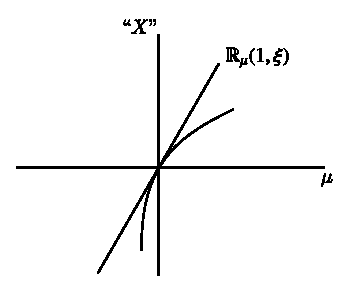
\includegraphics{figure/fig76-3.1.eps}
\caption{``regular point''}
\end{figure}

In this case, the origin is referred to as a {\em ``regular point''}. It is immediately checked that this is what happens in problems of bifurcation from the trivial branch when $\lambda_{0}$ is not a characteristic value of $L$. To sum up, in the first case, the {\em physical parameter} $\mu$ can also be used as a {\em mathematical parameter} for the parametrization of\pageoriginale the local zero set of $G$. The situtaion is different when (\ref{chap1-eq3.3}) holds instead of (\ref{chap1-eq3.2}). We can write
$$
Y = \mathbb{R}D_{\mu}G(0) \oplus Range D_{x}G(0),
$$
whereas
$$
\widetilde{X}_{1} = \Ker DG(0) = \{0\} \times \Ker D_{x}G(0) = \{0\} \times X_{1}.
$$

Since $\dim \widetilde{X}_{1} = 1$, we find $\dim X_{1} = 1$ and the local zero set of $G$ is a curve parametrized by $x_{1} \epsilon X_{1}$. It has a {\em ``vertical''} tangent at the origin, namely $\{0\} \times X_{1}$. Two typical situations are as follows:
\begin{figure}[H]
\centering
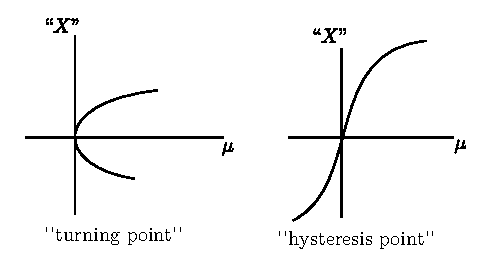
\includegraphics{figure/fig76-3.2.eps}
\caption{}
\end{figure}


\begin{remark}\label{chap1-rem3.1}
From a geometric point of view, there is no differences between a ``regular point'', a ``turning point'' or a ``hysteresis point'', since the last two become ``regular'' after a change of coordinates. But there is a difference in the number of solutions of the equation $G(\mu, x) = 0$ as the parameter $\mu$ changes sign.
\end{remark}

\begin{example*}
Given\pageoriginale an element $y^{0} \epsilon Y$, let us consider the equation 
\begin{equation*}
F(x) = \mu Y^{0}\tag{3.4}\label{chap1-eq3.4}
\end{equation*}
where $F : X \to Y$ is a mapping of class $C^{m}(m \geq 1)$ such that $F(0) = 0$. Setting $G(\mu, x) = F(x) - \mu y^{0}$, we are in the first case (i.e. $D_{x}G(0)$ is onto ) if $D_{x}F(0)$ is onto and the solutions are given by
$$
x = x(\mu), x(0) = 0,
$$
where $x(\cdot)$ is a mapping of class $C^{m}$ around the origin. Now, if codim Range $D_{x}F(0) = 1$ and $y^{0} \notin$ Range $D_{x}F(0)$, we are in the second case. The curve of solutions has a vertical tangent at the origin and it is not parametrized by $\mu$; as it follows from the above, a ``natural'' parameter is the one-dimensional variable of the space $\widetilde{X}_{1} = \Ker D_{x}F(0) \geq 1$ and $y^{0} \epsilon$ Range $D_{x}F(0)$, no conclusion can be drawn as yet.
\end{example*}

We shall now examine the case $n = 1$. Here the main tool will be the {\em Morse lemma}, of which we shall give two equivalent formulations.

\begin{theorem}\label{chap1-thm3.1}
(Morse lemma : ``strong'' version)\footnote{There is an veen stronger version that we shall, however, not use here.}: Let $f$ be a mapping of class $C^{m}, m \geq 2$ on a neighbourhood of the origin in $\mathbb{R}^{2}$ with values in $\mathbb{R}$, such that
$$
f(0) = 0.
$$
$$
Df(0) = 0,
$$\pageoriginale
$$
\text{ det } D^{2}f(0) \neq 0 \text{ (Morse condition).}
$$
Then, there is an origin-preserving $C^{m-1}$ local diffeomorphism $\phi$ in $\mathbb{R}^{2}$ with $D\phi(0) = I$ which transforms the local zero set of the quadratic form
$$
\widetilde{\xi} \epsilon \mathbb{R}^{2} \to D^{2} f (0). (\widetilde{\xi})^{2} \epsilon \mathbb{R}, 
$$
into the local zero set of $f$. Moreover, $\phi$ is $C^{m}$ away from the origin.
\end{theorem}

\begin{theorem*}[3.1']\label{chap1-thm3.1'}
(Morse lemma, ``weak'' version): Let $f$ be a mapping of class $C^{m}, m \geq 2$ on a neighbourhood of the origina in $\mathbb{R}^{2}$ with values in $\mathbb{R}$, verifying
\begin{align*}
& f(0) = 0,\\
& Df(0) = 0,\\
& det D^{2}f(0) \neq 0 (\text{Morse condition}).
\end{align*}

Then, the local zero set of $f$ reduces to the origin if det $D^{2}f(0) > 0$ and is made up of two curves of class $C^{m-1}$ if det $D^{2}f(0) < 0$. Moreover, these curves are of class $C^{m}$ away from the origin and each of them is tangent to a different one from among the two lines of the zero set of the quadratic form
$$
\widetilde{\xi} \epsilon \mathbb{R}^{2} \to D^{2}f(0) \cdot (\widetilde{\xi})^{2} \epsilon \mathbb{R},
$$
at the origin.
\end{theorem*}

\medskip
\noindent{\textit{NOTE}}\pageoriginale : We say that the curves {\em intersect transversally} at the origin.

\begin{comment}\label{chap1-com3.1}
By det $D^{2}f(0)$, we mean the determinant of the $2 \times 2$ matrix representing the second derivative of $f$ at the origin for a given basis of $\mathbb{R}^{2}$. Of course, this determinant depends on the basis (because the partial derivatives of $f$ do) but its {\em signs does not} (the proof of this assertion is simple and is left to the reader): the assumptions of Theorem \ref{chap1-thm3.1} and \ref{chap1-thm3.1}$'$ are {\em intrinsically linked to $f$}. In short, we shall say that the quadratic form $D^{2}f(0) \cdot (\widetilde{\xi})^2$ is non-degenerate.
\end{comment}

\begin{comment}\label{chap1-com3.2}
Theorem \ref{chap1-thm3.1} implies Theorem \ref{chap1-thm3.1}$'$, since the local zero set of the quadratic form
$$
\widetilde{\xi} \epsilon \mathbb{R}^{2} \to D^{2}f(0) \cdot (\widetilde{\xi})^{2} \epsilon \mathbb{R},
$$
reduces to the origin if det $D^{2}f(0) > 0$ (the quadratic form is then positive or negative definite) and is made up of exactly two distinct lines if det $D^{2}f(0) < 0$. If so, the local zero set of $f$ is the image of these two lines through the diffeomorphism $\phi$: it is then made up of two curves whose tangents at the origin are the images of the two lines in question through the linear isomorphism $D_{\phi}(0) = I$. We shall prove Theorem \ref{chap1-thm3.1}$'$ and that it implies Theorem \ref{chap1-thm3.1}$'$ in the next chapter, in a more general frame work.
\end{comment}
\begin{figure}[H]
\centering
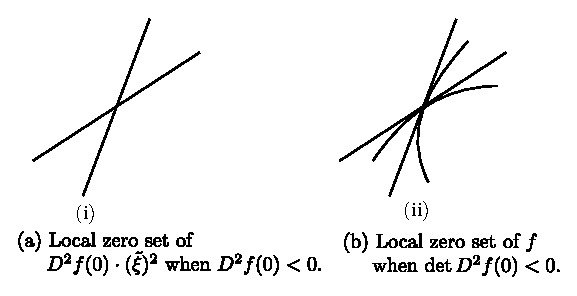
\includegraphics{figure/fig76-3.3.eps}
\caption{}
\end{figure}\pageoriginale

\begin{comment}\label{chap1-com3.3}
Theorem \ref{chap1-thm3.1} has a generalization to mappings from $\mathbb{R}^{n+1} \to \mathbb{R}, n \geq 1$. It is generally stated assuming $f \epsilon C^{m}, m \geq 3$ and the diffeomorphism $\phi$ is shown to be of class $C^{m-2}$ only (as in Nirenberg \cite{27}). This improved version is due to Kuiper \cite{21}. Infinite dimensional versions (cf. \cite{14, 28, 41}) are also available in this direction.
\end{comment}

\begin{comment}\label{chap1-com3.4}
In contrast, Theorem \ref{chap1-thm3.1}$'$ has a generalization to mapping from $\mathbb{R}^{n+1} \to \mathbb{R}^n$, which we shall prove in the next chapter. This will be a basic tool in Chapter \ref{chap3} where we study some general one-parameter problems.
\end{comment}

\begin{remark}\label{chap1-rem3.2}
There\pageoriginale is also a generalization of the {\em strong version} to mapping from $\mathbb{R}^{n+p} \to \mathbb{R}^{n}, p \geq 1$ at the expense of losing some regularity at the origin (cf. \cite{5}).
\end{remark}

{\em Application-first results.} Assume $n = 1$ in the Lyapunov-Schmidt reduction and let $f$ denote the reduced mapping. Since dim $\widetilde{X}_{1} = n+1 = 2$, $\dim Y_{1} = n = 1$ and the hypotheses of the Morse lemma are {\em independent of the system of coordinates}, we can identify $\widetilde{X}_{1}$ with $\mathbb{R}^{2}, Y_{1}$ with $\mathbb{R}$ so that $f$ becomes a mapping from a neighbourhood of the origin in $\mathbb{R}^{2}$ with values in $\mathbb{R}$. The conditions ; $f(0) = 0, Df(0) = 0$ are automatically fulfilled (cf. (\ref{chap1-eq2.10})). If, in addtion, det $D^{2}f(0) \neq 0$ (which requires $G$ to be of class $C^{2}$ at least) the structure of the local zero set of $f$, hence that of $G$ follows. In particular, {\em bifurcation occurs as soon} as det $D^{2}f(0) = 0$.

\begin{remark}\label{chap1-rem3.3}
The independence of the hypotheses of the Morse Lemma on the system of coordinates does not prove that they are independent of the spaces $X_{2}$ and $Y_{1}$. However, such a result is true as we shall see later, in this section.
\end{remark}

\medskip
\noindent{\textbf{New formulation of the Morse lemma}}: We shall prove that the Morse condition has an {\em equivalent formulation} which will be basic for further generalizations.

\begin{lemma}\label{chap1-lem3.1}
Let $f$ be as in the Morse lemma. Then the Morse condition det $D^{2}f(0) \neq 0$ is equivalent to the following property: For every $\widetilde{\xi} \epsilon \mathbb{R}^{2} - \{0\}$\pageoriginale such that $D^{2}f(0).(\widetilde{\xi})^{2} = 0$, the linear form $D^{2}f(0) \cdot\tilde{\xi} \mathscr{L} (\mathbb{R}^{2}, \mathbb{R})$ is onto.
\end{lemma}

\begin{proof}
As $f$ is a mapping from $\mathbb{R}^{2}$ into $\mathbb{R}$. its derivative $Df$ is a mapping from $\mathbb{R}^{2}$ into the space $\mathscr{L} (\mathbb{R}^{2}, \mathbb{R}) \simeq \mathbb{R}^{2}$. Hence
$$
D^{2}f(0) \epsilon \mathscr{L} (\mathbb{R}^{2}, \mathscr{L} (\mathbb{R}^{2}, \mathbb{R})) \simeq \mathscr{L} (\mathbb{R}^{2}, \mathbb{R}^{2})
$$
and saying that det $D^{2}f(0) \neq 0$ means that $\Ker D^{2}f(0) = \{0\}$, i.e. for every $\widetilde{\xi} \epsilon \mathbb{R} - \{0\}, D^{2}f(0) \cdot \widetilde{\xi} \neq 0$. But this last condition is certainly fulfilled by those elements $\widetilde{\xi}$ such that $D^{2}f(0) \cdot (\widetilde{\xi})^{2} \neq 0$ (regardless of the condition det $D^{2}f(0) \neq 0$) and it is then not restrictive to write

det $D^{2}f(0) \neq 0 \Leftrightarrow \{D^{2}f(0) \cdot \widetilde{\xi} \neq 0$ for very $\widetilde{\xi} \epsilon \mathbb{R} - \{0\}$ such that $D^{2}f(0) \cdot (\widetilde{\xi})^{2} \neq 0\}$ .

The result follows from the obvious fact that a linear form is onto if and only ifi it is not the zero form.
\end{proof}

With the above lemma, we get equivalent version of the ``weak'' Morse lemma.

\begin{theorem*}[3.1$''$]\label{chap1-thm3.1''}
Let $f$ be a mapping of class, $C^{m} \geq 2$ on a neighbourhood of the origin in $\mathbb{R}^{2}$ with values in $\mathbb{R}$, verifying
\begin{align*}
& f(0) = 0,\\
& Df(0) = 0,
\end{align*}
such that the linear form $D^{2}f(0) \cdot \widetilde{\xi} \in \mathscr{L} (\mathbb{R}^{2}, \mathbb{R})$ is onto for every $\tilde{\xi} \in \mathbb{R}^2 - \{0\}$ with $D^2 f (0) \cdot (\tilde{\xi})^2 = 0$. Then the local zero set od the quadratic\pageoriginale form $D^{2}f(0) \cdot (\widetilde{\xi})^{2}$ consists of exactly 0 or 2 real lines (depending on the sign of det $D^{2}f(0)$) and the local zero step of $f$ is made up of the same number of $C^{m-1}$ curves through the origin. Moreover, these curves are of class $C^{m}$ away from the origin and each of them is tangent to a different one from among the lines in the zero of the quadractic form $D^{2}f(0) \cdot \widetilde{\xi}^(2)$ at the origine.
\end{theorem*}


\medskip
\noindent{\textit{Application - further details}}. Assume that $n = 1$  in the 
Lyapunov-Schmidt reduation and let $f$ denoted the reduced mapping. From the 
exposition of Theorem 3.1$''$, it does not matter if $\mathbb{R}^{2}$ and $\mathbb{R}$ are replaced by the space $\widetilde{X}_{1}$ and $Y_{1}$ respectively. Since $f(0) = 0$ and $Df(0) = 0$, it remains to check whether the Morse condition holds. By definition of $f$ (cf.(\ref{chap1-eq2.9})) we first find, for every $\widetilde{\xi} \epsilon \widetilde{X}_{1}$, that
$$
Df(\widetilde{x}) \cdot \widetilde{\xi} = Q_{1} DG(\widetilde{x} + \widetilde{\varphi}(\widetilde{x})) \cdot (\widetilde{\xi} + D\widetilde{\varphi}(\widetilde{x}) \cdot \widetilde{\xi}).
$$

Since $\widetilde{\varphi}(0) = 0$ and $D\widetilde{\varphi}(0) = 0$ (cf. (\ref{chap1-eq2.12})), we obtain
$$
D^{2}f(0) \cdot (\widetilde{\xi})^{2} = Q_{1}D^{2}G(0) \cdot (\widetilde{\xi})^{2} + Q_{1}DG(0) \cdot (D^{2} \widetilde{\varphi}(0) \cdot (\widetilde{\xi})^{2}).
$$

But $Q_{1}DG(0) = 0$, by the definition of $Q_{1}$ and hence
\begin{equation*}
D^{2}f(0). (\widetilde{\xi})^{2} = Q_{1}D^{2}G(0) \cdot (\widetilde{\xi})^{2}.
\end{equation*}
a particularly simple expression in terms of the mapping $G$.

We now prove
\begin{theorem}\label{chap1-thm3.2}
The validity of the Morse condition for the reduced mapping\pageoriginale $f$  is independent of the choice of the spaces $\widetilde{X}_{2}$ and $Y_{1}$.
\end{theorem}

\begin{proof}
Clearly, the mapping
$$
\widetilde{\xi} \epsilon \widetilde{X}_{1} \to Q_{1}D^{2}G(0) \cdot (\widetilde{\xi})^{2} \epsilon Y_{1},
$$
is independent of the space $\widetilde{X}_{2}$ and it remains to show that the required property of surjectivity is independent of $Y_{1}$ as well. Let us then assume that the property holds and let $\hat{Y}_{1}$ be another complement of $Y_{2}$. Denoting by $\hat{Q}_{1}$ and $\hat{Q}_{2}$ the associated projection operators, we must show that the linear form $\hat{Q}_{1}D^{2}G(0) \cdot \widetilde{\xi}$ is nonzero for every $\widetilde{\xi} \epsilon \widetilde{X}_{1} - \{0 \}$ such that $\hat{Q}_{1}D^{2}G(0) \cdot (\widetilde{\xi})^{2} = 0$.

First, note that $\hat{Q}_{1}$ is an {\em isomorphism} of $Y_{1}$ to $\hat{Y}_{1}$. Indeed, both spaces have the same dimension and it suffices to prove that the restriction of $\hat{Q}_{1}$ to $Y_{1}$ is one-to-one. If $\hat{Q}_{1} y_{1} = 0$ for some $y_{1} \epsilon Y_{1}$, we must have $y_{1} \epsilon Y_{2}$ (since $\Ker \hat{Q}_{1} - Y_{2}$) and hence $y_{1} \epsilon Y_{1} \cap Y_{2} = \{0\}$. Next, observe that
\begin{equation*}
\hat{Q}_{1} = \hat{Q}_{1} Q_{1}.\tag{3.6}\label{chap1-eq3.6}
\end{equation*}

Indeed, one has $\hat{Q}_{1} Q_{1} = \hat{Q}_{1}(I - Q_{2}) = \hat{Q}_{1} - \hat{Q}_{1} Q_{2}$. But $\hat{Q}_{1} Q_{2} = 0$ (since $\Ker \hat{Q}_{1} = Y_{2}$ again), which proves (\ref{chap1-eq3.6}).

Let then $\widetilde{\xi} \epsilon \widetilde{X}_{1} - \{0\}$ be such that $\hat{Q}_{1}D^{2}G(0) \cdot (\widetilde{\xi})^{2} = 0$.

From (\ref{chap1-eq3.6}), this can be written as
$$
\hat{Q}_{1} Q_{1} D^{2}G(0) \cdot (\widetilde{\xi})^{2} = 0.
$$

As $\hat{Q}_{1} \epsilon$ Isom $(Y_{1}, \hat{Y}_{1})$, we find
$$
Q_{1}D^{2}G(0) \cdot (\widetilde{\xi})^{2} = 0.
$$\pageoriginale

But, from our assumptions, $Q_{1}D^{2}G(0) \cdot \widetilde{\xi} \neq 0$. By the same argument of isomorphism, $\hat{Q}_{1} Q_{1} D^{2}G(0) \cdot \widetilde{\xi} \neq 0$ and using (\ref{chap1-eq3.6}) again we finally see that
$$
\hat{Q}_{1} D^{2}G(0) \cdot \widetilde{\xi} \neq 0,
$$
which completes the proof.
\end{proof}

\medskip
\noindent{\textit{Practical Method}}: Let $y^{0}$ be any nonzero element of the space $Y_{1}^{-}$ and let $y^{*} \epsilon Y'$ (topological dual of $Y$) be characterized by
\begin{equation*}
\begin{cases}
&  \langle y^{*} , y \rangle = 1,\\
&  \langle y^{*} , y \rangle = 0 \text{ for every } y \epsilon Y_{2}
\end{cases}\tag{3.7}\label{chap1-eq3.7}
\end{equation*}
(The existence of such an element $y^{*}$ is ensured by the Hahn-Banach theorem). Then, for every $y \epsilon Y$.
\begin{equation*}
Q_{1}y = \langle y^{*}, y \rangle y^{0}.\tag{3.8}\label{chap1-eq3.8}
\end{equation*}

\begin{remark}\label{chap1-rem3.4}
One may object that using the Hahn-Banach theorem is ``practical''. Actually, using the linear form $y^{*}$ is only a convenient way to get explicit formulation of the projection operator $Q_{1}$, which is the important thing to know in practice.
\end{remark}

It follows, for every $\widetilde{\xi} \epsilon \widetilde{X}_{1}$, that
$$
D^{2}f(0) \cdot (\widetilde{\xi})^{2} = Q_{1}D^{2}G(0) \cdot (\widetilde{\xi})^{2} = \langle y^{*}, D^{2}G(0) \cdot (\widetilde{\xi})^{2} \rangle y^{0}.
$$

Now\pageoriginale let $(\widetilde{e}_{1}, \widetilde{e}_{2})$ be a basis of $\widetilde{X}_{1}$ so that $\widetilde{\xi} \epsilon \widetilde{\xi}_{1}$ writes
$$
\widetilde{\xi} = \xi_{1} e_{1} + \xi_{2} e_{2} , \xi_{1}, \xi_{2} \epsilon \mathbb{R}.
$$

Then 
\begin{align*}
Q_{1}D^{2}G(0) \cdot (\widetilde{\xi})^{2} & = [\xi_{1}^{2} \langle y^{*}, D^{2}G(0) \cdot (\widetilde{e}_{1})^{2} \rangle + 2 \xi_{1} \xi_{2} \langle y^{*}, D^{2}G(0) \cdot (\widetilde{e}_{1}, \widetilde{e}_{2}) \rangle \\
& +\xi_{2}^{2} \langle y^{*}, D^{2}G(0) \cdot (\widetilde{e}_{2})^{2} \rangle ] y^{0}
\end{align*}
and the above mapping veriies the Morse condition if and only if the quadratic form
\begin{align*}
(\xi_{1}, \xi_{2}) \epsilon \mathbb{R}^{2} \to & [\xi_{1}^{2}  \langle y^{*}, D^{2}G(0) \cdot (\widetilde{e}_{1})^{2} \rangle + 2 \xi_{1} \xi_{2}  \langle y^{*}, D^{2}G(0) \cdot (\widetilde{e}_{1}, \widetilde{e}_{2}) \rangle \\
& + \xi_{2}^{2} \langle y^{*} , D^{2}G(0) \cdot (\widetilde{e}_{2})^{2}  \rangle ] \epsilon \mathbb{R},\tag{3.9}\label{chap1-eq3.9}
\end{align*}
is non-degenerate, i.e. the discriminant
\begin{equation*}
\langle y^{*}, D^{2}G(0) \cdot (\widetilde{e}_{1}, \widetilde{e}_{2}) \rangle^{2} - \langle y^{*}, D^{2}G(0) \cdot (\widetilde{e}_{1})^{2} \rangle \langle y^{*}, D^{2}G(0) \cdot (\widetilde{e}_{2})^{2}  \rangle \tag{3.10}\label{chap1-eq3.10}
\end{equation*}
is non zero.

\begin{remark}\label{chap1-rem3.5}
Note that the {\em discriminant} (\ref{chap1-eq3.10}) is just $(-1)$ times of the {\em determinant} of the quadratic form (\ref{chap1-eq3.9}).
\end{remark}

{\em The example of problems of bifurcation from the trivial branch at a geometrically simple characteristic value.}

Let $G(\mu, x) = 0$ be a problem of bifurcation from the trivial branch (cf. (\ref{chap1-eq1.6})) with {\em compact} operator $L \epsilon \mathscr{L}(X)$ and nonlinear part $\Gamma \epsilon C^{m}$ with $m \geq 2$, the real number $\lambda_{0}$ being a characteristic\pageoriginale  value of $L$ (the obvious case when $\lambda_{0}$ is not a characteristic value of $L$ has already been considered). As we know
\begin{align*}
\widetilde{X}_{1} & = \mathbb{R} \times \Ker (I - \lambda_{0}L) \subset \mathbb{R} \times X,\\
Y_{2} & = Range (I - \lambda_{0}L) \subset X(= Y),
\end{align*}
so that $n = codim Y_{2} = 1$ if and only if $\dim \Ker (I - \lambda_{0}L) = 1$ i.e. the characteristic value $\lambda_{0}$ is {\em geometrically simple}.

Since
$$
G(\mu, x) = (I - (\lambda_{0} + \mu) L) x + \Gamma(\mu, x),
$$
we find, from (\ref{chap1-eq1.7}) and (\ref{chap1-eq1.9}), that
\begin{align*}
& D_{\mu}^{2}G(0) = 0\\
& D_{\mu}D_{x}G(0) = -L + D_{\mu} D_{x} \Gamma (0) = -L
\end{align*}
and
$$
D_{x}^{2}G(0) = D_{x}^{2}\Gamma(0).
$$

As a result, for $(\mu, x) \epsilon \mathbb{R} \times X$
$$
D^{2}G(0) \cdot (\mu, x)^{2} = -2\mu L x + D_{x}^{2} \Gamma(0) \cdot (x)^{2}.
$$

In particular, for $x \epsilon X_{1}$, one has $Lx = (1/ \lambda_{0})x$, so that
$$
Q_{1}D^{2}G(0) \cdot (\mu, x)^{2} = -\frac{2}{\lambda_{0}} \mu Q_{1} x + Q_{1}D_{x}^{2}G(0) \cdot (x)^{2},
$$
for $(\mu, x) \epsilon \mathbb{R} \times \Ker (I - \lambda_{0}L)$.

Given any $x^{0} \epsilon \Ker (I - \lambda_{0} L) - \{0\}$, the pair $((1, 0), (0, x^{0}))$ is a basis of $\mathbb{R} \times \Ker (I - \lambda_{0}L)$. The practical method described before leads\pageoriginale to the examination of the sign of the determinant of the quadratic polynomial
\begin{equation*}
(\mu, t) \epsilon \mathbb{R}^{2} \to \frac{-2\mu t}{\lambda_{0}} \langle y^{*}, x^{0} \rangle + t^{2} \langle y^{*}, D_{x}^{2} \Gamma(0) \cdot (x^{0})^{2} \rangle,\tag{3.11}\label{chap1-eq3.11}
\end{equation*}
where $y^{*} \epsilon X'$ is some linear continuous form with null space $Y_{2}$. The discriminant of the polynomial (\ref{chap1-eq3.11}) is
$$
\frac{4}{\lambda_{0}^{2}} \langle y^{*}, x^{0} \rangle^{2} \geq 0.
$$

It is positive if and only if $\langle y^{*}, x^{0}  \rangle \neq 0$, namely $x^{0} \notin Y_{2}$. As $\Ker (I - \lambda_{0}L) = \mathbb{R} x^{0}$ and $Y_{2} = Range (I - \lambda_{0}L)$, this means that $\Ker (I - \lambda_{0}L) \nsubset Range (I - \lambda_{0}L)$. But, if so, (as codim Range $(I - \lambda_{0}L) = \dim \Ker (I - \lambda_{0}L) = 1$, by hypothesis) we deduce that
\begin{equation*}
X = \Ker (I - \lambda_{0}L) \oplus Range (I - \lambda_{0}L)\tag{3.12}\label{chap1-eq3.12}
\end{equation*}
which expresses that the characterstic value $\lambda_{0}$ is also {\em algebraically simple}.

To sum up, the Morse lemma applies to problems of bifurcation from the trivial branch at a {\em geometrically simple} eigenvalue $\lambda_{0}$ if and only if $\lambda_{0}$ is also {\em algebraically simple}. Then, the local zero set of the reduced mapping and hence that of $G$ consists of the union of the trivial branch and a {\em second branch} (curve of class $C^{m-1}$ at the origin and of class $C^{m}$ away from it) bifurcating from the trivial\pageoriginale branch at the origin.
\begin{figure}[H]
\centering
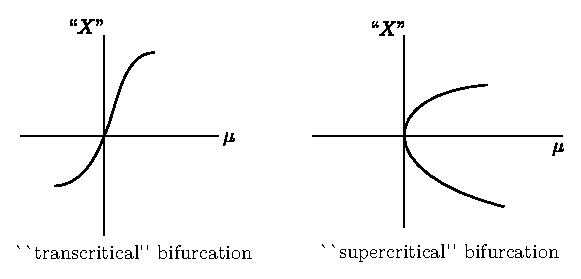
\includegraphics{figure/fig76-3.4.eps}
\caption{Local zero set of $G$.}
\end{figure}

\begin{remark}\label{chap1-rem3.6}
These conclusions agree with Krasnoselskii's Theorem (Theorem \ref{chap1-thm1.2}) but provide much more precise information on the {\em structure} of the local zero set. This result was originally proved by Crandall and Rabinowitz (\cite{7}) in a different way involving the application of the Implict function theorem, {\em after a modification of the reduced equation}. This method uses the fact that the trivial branch is in the local zero set of $G$ explicitly. Note that the same result holds (with the same proof) when the more general conditions $\Gamma(\mu, 0) = 0, D_{x} \Gamma(0) = 0$ and $Q_{1}D_{\mu}D_{x} \Gamma(0) = 0$ replace (\ref{chap1-eq1.7})-(\ref{chap1-eq1.9}).
\end{remark}

\begin{remark}\label{chap1-rem3.7}
The complementary case $\Ker (I - \lambda_{0}L) \subset Range(I - \lambda_{0}L)$, namely, when the characteristic value $\lambda_{0}$ is {\em geometrically simple} in\break which the Morse condition fails (referred to as a {\em ``degenerate case''}) will be considered in Chapter \ref{chap5}.
\end{remark}
